\whiteBGstarBegin
\setcounter{section}{0}
\section{Trắc nghiệm}
\begin{enumerate}[label=\bfseries Câu \arabic*:]
	
	\item \mkstar{1}
	
	\cauhoi
	{Điều kiện cân bằng của vật rắn chịu tác dụng của ba lực không song song là
		\begin{mcq}
			\item hợp lực của hai lực phải bằng lực thứ 3.
			\item hợp lực của hai lực phải cân bằng với lực thứ 3.
			\item hợp lực của hai lực phải lớn hơn lực thứ 3.
			\item tổng hai lực phải bằng lực thứ 3.
		\end{mcq}
	}
	
	\loigiai
	{	\textbf{Đáp án: B.}
		
		Điều kiện cân bằng của vật rắn chịu tác dụng của ba lực không song song là hợp lực của hai lực phải cân bằng với lực thứ 3.
	}
	
	\item \mkstar{2}
	
	\cauhoi
	{Một vật chịu tác dụng của hai lực: $\vec F_1$ và $\vec F_2$. Lực $\vec F_1$ nằm ngang hướng sang phải, độ lớn $\SI{10}{N}$. Để vật ở trạng thái cân bằng thì lực $\vec F_2$ có đặc điểm là
		\begin{mcq}
			\item cùng giá, cùng chiều, có độ lớn $\SI{10}{N}$.
			\item nằm ngang, hướng sang trái, có độ lớn $\SI{10}{N}$.
			\item nằm ngang, hướng sang phải, có độ lớn $\SI{10}{N}$.
			\item cùng giá, hướng sang trái, độ lớn $\SI{10}{N}$.
		\end{mcq}
	}
	
	\loigiai
	{	\textbf{Đáp án: D.}
		
	Để vật ở trạng thái cân bằng thì lực $\vec F_2$ có đặc điểm là cùng giá, hướng sang trái, độ lớn $\SI{10}{N}$.
	}
	\item \mkstar{2}
	
	\cauhoi
	{Ba lực đồng phẳng, đồng quy tác dụng lên một vật rắn nằm cân bằng có độ lớn lần lượt là $\SI{12}{N}$, $\SI{16}{N}$ và $\SI{20}{N}$. Nếu lực $\SI{16}{N}$ không tác dụng vào vật nữa, thì hợp lực tác dụng lên nó là
		\begin{mcq}(4)
			\item $\SI{16}{N}$.
			\item $\SI{20}{N}$.
			\item $\SI{15}{N}$.
			\item $\SI{12}{N}$.
		\end{mcq}
	}
	
	\loigiai
	{	\textbf{Đáp án: A.}	
		
	Vật rắn nằm cân bằng nên
	$$F_1 + F_2 = F_3 = \SI{16}{N}$$
	}
	
	
	
	\item \mkstar{4}
	
	\cauhoi
	{Một ngọn đèn có khối lượng $m=\SI{1}{kg}$ được treo dưới trần nhà bằng một sợi dây. Người ta đã treo đèn này bằng cách luồn sợi dây qua một cái móc của đèn và hai đầu dây được gắn chặt trên trần nhà (hình vẽ).
		\begin{center}
			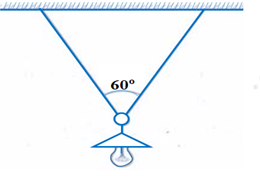
\includegraphics[scale=1]{../figs/VN10-2021-PH-TP020-7.png}
		\end{center}
	
	Hai nửa sợi dây có chiều dài bằng nhau và hợp với nhau một góc bằng $60^\circ$. Hỏi lực căng của mỗi nửa sợi dây là bao nhiêu?
		\begin{mcq}(4)
			\item $\SI{5.66}{N}$.
			\item $\SI{11.32}{N}$.
			\item $\SI{4.66}{N}$.
			\item $\SI{3.77}{N}$.
		\end{mcq}
	}
	
	\loigiai
	{	\textbf{Đáp án: A.}
		
	Khi ngọn đèn nằm cân bằng thì
	$$\vec P + \vec T+1 + \vec T_2 = 0 \Rightarrow \vec P + \vec T = 0 \Rightarrow P = T = \SI{9,8}{N}$$
	
	Mà $T=2T_1 = \cos (30^\circ) = \sqrt{3} T_1 \Rightarrow T_1 = T_2 = \dfrac{T}{\sqrt{3}} = \SI{5.66}{N}$.
	}
	
	\item \mkstar{4}
	
	\cauhoi
	{Một quả cầu đồng chất có khối lượng $\SI{3}{kg}$ được treo vào tường nhờ một sợi dây. Dây làm với tường một góc $\alpha = 20^\circ$ (hình vẽ).
		\begin{center}
			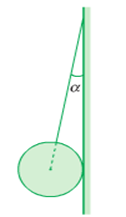
\includegraphics[scale=1]{../figs/VN10-2021-PH-TP020-6.png}
		\end{center}
		
	Bỏ qua ma sát ở chỗ tiếp xúc của quả cầu với tường. Lấy $g=\SI{10}{m/s^2}$. Lực căng $T$ của dây là bao nhiêu?	
		\begin{mcq}(4)
			\item $\SI{88}{N}$.
			\item $\SI{10}{N}$.
			\item $\SI{22}{N}$.
			\item $\SI{32}{N}$.
		\end{mcq}
	}
	
	\loigiai
	{	\textbf{Đáp án: D.}
		
	Khi quả cầu ở trạng thái cân bằng, không có ma sát thì tổng hợp các lực tác dụng lên quả cầu tuân theo quy tắc tổng hợp các lực không song song tác dụng lên một vật cân bằng: 
	%------------------
	\begin{equation*}
		\vec{P}+\vec{N}+\vec{T}=\vec{0}
		\Leftrightarrow 
		\vec{P}+\vec{N}=\vec{T}=-\vec{T}'.
	\end{equation*}
	%-------------------
	Nhìn trên hình vẽ, ta cũng có thể thấy rằng lực $\vec{T}'$ hợp với lực $\vec{P}$ một góc $\alpha=20^{\circ}$. Từ đó, ta có:
	\begin{equation*}
		\cos\alpha =\dfrac{P}{T'}
		\Rightarrow
		T'=\dfrac{P}{\cos\alpha}
		=
		\dfrac{\SI{30}{N}}{\cos 20^{\circ}}
		\approx 
		\SI{32}{N}.
	\end{equation*}
	%--------------
	Vì $T=T'$ nên độ lớn lực căng dây là: $T=\SI{32}{N}$.
	}
	
\end{enumerate}

\whiteBGstarEnd

\loigiai
{
	\begin{center}
		\textbf{BẢNG ĐÁP ÁN}
	\end{center}
	\begin{center}
		\begin{tabular}{|m{2.8em}|m{2.8em}|m{2.8em}|m{2.8em}|m{2.8em}|m{2.8em}|m{2.8em}|m{2.8em}|m{2.8em}|m{2.8em}|}
			\hline
			1.B  & 2.D  & 3.A  & 4.A  & 5.D  & & & & &  \\
			\hline
			
		\end{tabular}
	\end{center}
}
\section{Tự luận}
\begin{enumerate}[label=\bfseries Câu \arabic*:]
	\item \mkstar{1}
	
	\cauhoi{
		Phát biểu điều kiện cân bằng của một vật rắn chịu tác dụng của hai lực. Điều kiện cân bằng của một vật chịu tác dụng của ba lực không song song là gì?
	}
	
	\loigiai{
		
		Điều kiện cân bằng của một vật rắn chịu tác dụng của hai lực là hai lực đó phải cùng giá, cùng độ lớn và ngươc chiều.
		$$\vec F_1 + \vec F_2 = 0$$
		hay
		$$\vec F_1 = - \vec F_2$$
		
		Điều kiện cân bằng của một vật chịu tác dụng của ba lực không song song:
		\begin{itemize}
			\item Ba lực đó phải có giá đồng phẳng và đồng quy;
			\item Hợp lực của hai lực phải cân bằng với lực thứ ba: $\vec F_1 + \vec F_2 = - \vec F_3$.
		\end{itemize}
	}
	
	\item \mkstar{2}
	
	\cauhoi
	{Cho biết trọng tâm của một số vật đồng chất và có dạng hình học đối xứng.
	}
	
	\loigiai
	{
	Đối với những vật phẳng mỏng có dạng hình học đối xứng (hình tròn, tam giác đều, hình vuông, hình chữ nhật) thì trọng tâm chính là tâm đối xứng của vật.
	}
	\item \mkstar{3}
	
	\cauhoi
	{Một vật có khối lượng $m=\SI{2}{kg}$ được giữ yên trên một mặt phẳng nghiêng bởi một sợi dây song song với đường dốc chính (hình vẽ).
		\begin{center}
			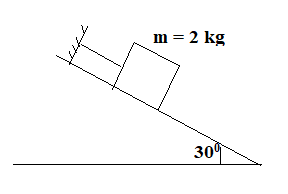
\includegraphics[scale=0.8]{../figs/VN10-2021-PH-TP020-1.png}
		\end{center}
		 Biết góc nghiêng $\alpha=30^\circ$, $g=\SI{9.8}{m/s^2}$ và ma sát là không đáng kể. Hãy xác định:
		\begin{enumerate}
			\item Lực căng của dây;
			\item Phản lực của mặt phẳng nghiêng lên vật.
		\end{enumerate}
	}
	
	\loigiai
	{Các lực tác dụng lên vật gồm: trọng lực $\vec P$, phản lực $\vec N$ và lực căng dây $\vec T$.
		
	Khi vật cân bằng, ta có:
	$$\vec P + \vec F + \vec N = 0$$
	
	Trên phương $\text Ox$: $P_x - T = 0$.
	
	Trên phương $\text O y$: $-P_y + N = 0$.
	\begin{enumerate}
		\item Lực căng của dây;
		
	Lực căng dây $T=P_x = P \sin \alpha = \SI{9.8}{N}$
	
		\item Phản lực của mặt phẳng nghiêng lên vật.
		
	Phản lực của mặt phẳng nghiêng lên vật: $N=P_y = P \cos \alpha = \SI{16.97}{N}$.
	\end{enumerate}
	}
	\item \mkstar{4}
	
	\cauhoi
	{Một quả cầu có trọng lượng $P=\SI{40}{N}$ được treo vào tường nhờ một sợi dây hợp với mặt tường một góc $\alpha=30^{\circ}$. 
				\begin{center}
			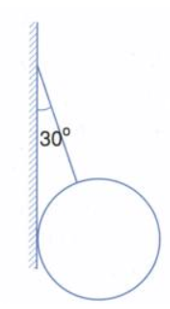
\includegraphics[scale=0.8]{../figs/VN10-2021-PH-TP020-2.png}
		\end{center}
		Bỏ qua ma sát ở chỗ tiếp xúc giữa quả cầu và tường, hãy xác định lực căng dây tác dụng lên quả cầu. 
	}
	
	\loigiai
	{Nhìn vào hình vẽ, ta thấy các lực tác dụng lên vật ở trạng thái cân bằng bao gồm: 
		\begin{itemize}
			\item lực căng dây $\vec{T}$ do sợi dây treo tác dụng lên vật, 
			\item trọng lực $\vec{P}$ tác dụng lên khối tâm của vật, 
			\item phản lực $\vec{N}$ do bức tường tác dụng lên vật.
		\end{itemize}
		\begin{center}
			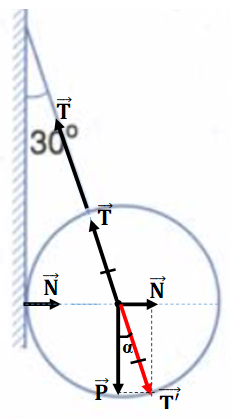
\includegraphics[scale=0.5]{../figs/VN10-2021-PH-TP020-3.png}
		\end{center}
		%---------------------------------
		Khi quả cầu ở trạng thái cân bằng, không có ma sát thì tổng hợp các lực tác dụng lên quả cầu tuân theo quy tắc tổng hợp các lực không song song tác dụng lên một vật cân bằng: 
		%------------------
		\begin{equation*}
			\vec{P}+\vec{N}+\vec{T}=\vec{0}
			\Leftrightarrow 
			\vec{P}+\vec{N}=\vec{T}=-\vec{T}'.
		\end{equation*}
		%-------------------
		Nhìn trên hình vẽ, ta cũng có thể thấy rằng lực $\vec{T}'$ hợp với lực $\vec{P}$ một góc $\alpha=30^{\circ}$. Từ đó, ta có:
		\begin{equation*}
			\cos\alpha =\dfrac{P}{T'}
			\Rightarrow
			T'=\dfrac{P}{\cos\alpha}
			=
			\dfrac{\SI{40}{N}}{\cos 30^{\circ}}
			\approx 
			\SI{46,2}{N}.
		\end{equation*}
		%--------------
		Vì $T=T'$ nên độ lớn lực căng dây là: $T=\SI{46,2}{N}$.
	}
	\item \mkstar{4}
	
	\cauhoi
	{Hai mặt phẳng đỡ tạo với mặt phẳng nằm ngang các góc $45^{\circ}$.Trên hai mặt phẳng đó người ta đặt một quả tạ hình cầu có khối lượng $\SI{5}{kg}$. Bỏ qua ma sát và lấy $g=\SI[parse-numbers=false]{10}{m/s^2}$. Hỏi áp lực của quả cầu lên mỗi mặt phẳng đỡ bằng bao nhiêu?
		\begin{center}
			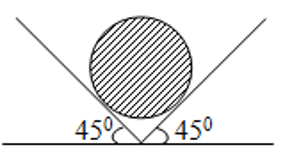
\includegraphics[scale=0.8]{../figs/VN10-2021-PH-TP020-5.png}
		\end{center}
	}
	
	\loigiai
	{Gọi $\vec{N}_1$ và $\vec{N}_2$ là phản lực do hai mặt phẳng tác dụng lên quả cầu và $\vec{P}'$ là lực trực đối với trọng lực $\vec{P}$. Vẽ các lực, ta được như hình sau 
		%--------%
		\begin{center}
			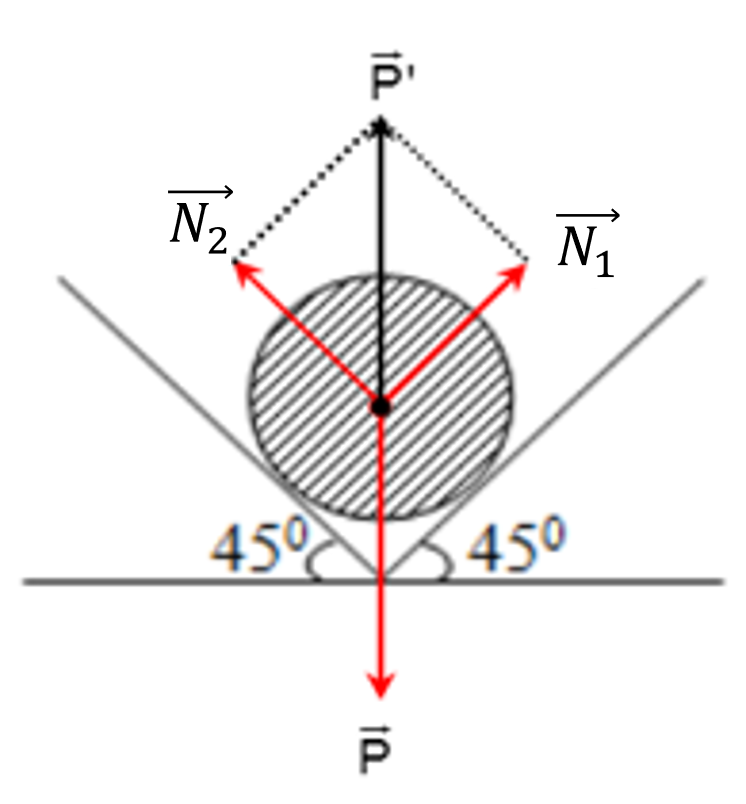
\includegraphics[scale=0.3]{../figs/VN10-2021-PH-TP020-4.png}
		\end{center}
		%---------------%
		Áp dụng điều kiện cân bằng của một vật dưới tác dụng của ba lực không song song ta có liên hệ:
		%------------%%%%
		\begin{equation*}
			\vec{N}_1 + \vec{N}_2 + \vec{P}  =\vec{0}. 
		\end{equation*}
		%-----------------%%%%%%
		Do $\vec{P}'=-\vec{P}$ nên ta suy ra được liên hệ: 
		\begin{equation*}
			\vec{N}_1 + \vec{N}_2 = \vec{P}'=-\vec{P}.
		\end{equation*}
		%%---------%%%% 
		Nhìn trên hình, ta thấy rằng giá của hai vectơ phản lực song song với hai mặt phẳng và vì vậy hợp với giá của $\vec{P}'$ góc $45^{\circ}$, nên có thể tính ra được độ lớn của phản lực qua công thức: 
		\begin{align*}
			N_1&=N_2=P'\cdot \cos 45^\circ=P\cdot \cos 45^\circ = m\cdot g \cdot \cos 45^\circ\\
			&=
			\SI{5}{kg}\cdot \SI[parse-numbers=false]{10}{m/s^2} \cdot \cos 45^\circ \\
			&=
			\SI[parse-numbers=false]{25\sqrt{2}}{N}. 
		\end{align*}	
		%--------------%
		Vậy độ lớn của hai phản lực bằng nhau và bằng $	\SI[parse-numbers=false]{25\sqrt{2}}{N}$.
	}
\end{enumerate}